\chapter{Implantação}
\label{cap6}

A implantação refere-se ao modo como os microsserviços foram executados, levando em conta o seu ambiente, caracteristicas da rede, serviços auxiliares e modelo de automatização utilizado.
%
Neste modelo pode-se também adicionar o modo de armazenamento e obtenção dos dados da execução dos testes.

A fim de permitir a reprodução do experimento em um ambiente com as mesmas características, a Seção~\ref{sec:ambiente} descreve o ambiente, segregando em sub-redes, tal qual as sub-redes de microsserviços, clientes, métricas e banco de dados.


\section{Ambiente}
\label{sec:ambiente}

O ambiente de testes foi dividido em dois sub-ambientes, a fim de controlar a conexão entre o cliente e a arquitetura de microsserviços fisicamente.
%
Dessa forma, obriga-se a utilização da rede para a conexão entre ambos.
%
Em especial foram implantados três ambientes distintos na núvem computacional Tchê (UDESC), tendo uma separação física entre os clientes e serviços de acesso.
%
O ambiente virtual implantado pode ser visualizado na Figura~\ref{fig:network_open_stack}.

\begin{figure}[htb!]
  \caption{Rede virtual criada no ambiente OpenStack}
  \label{fig:network_open_stack}
  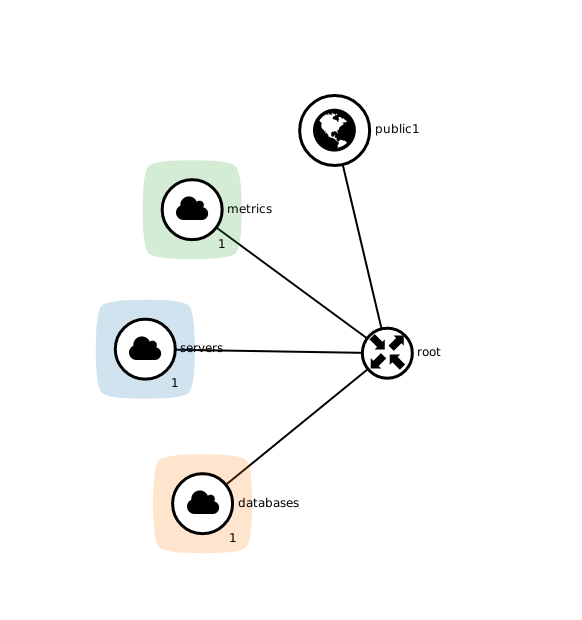
\includegraphics[width=0.8\textwidth]{figuras/network/circles_only_networks.png}
  \centering

  Fonte: O próprio autor.
\end{figure}

Os ambientes implantados, visíveis na Figura~\ref{fig:network_open_stack}, foram:

\begin{itemize}
  \item \textit{servers}: Ambiente de microsserviços;
  \item \textit{databases}: Ambiente de dados; e
  \item \textit{metrics}: Ambiente de métricas.
\end{itemize}

O ambiente de microsserviços foi implantado em um ambiente virtualizado sobre uma nuvem OpenStack.
%
Esta implantação é detalhada na Subseção~\ref{sec:ambiente_mic}.

O ambiente de dados é um ambiente próximo ao ambiente de microsserviços, porém não existe a necessidade de sua reinicialização da máquina virtual a cada teste. Por este motivo, além de ser uma boa prática de segurança para não expor o banco de dados a rede, os serviços de armazenamento de dados foram implantados em uma sub-rede a parte, utilizando Docker Compose.
%
Esta implantação é detalhada na Subseção~\ref{sec:ambiente_db}.

O ambiente de clientes foi implantado em um laboratório de computadores, sobre o sistema de gestão de contêineres Docker Swarm.
%
Esta implantação é detalhada na Subseção~\ref{sec:ambiente_cli}.

Durante a execução dos testes, ambos os ambientes  de microsserviços e clientes enviam dados ao serviço de métricas, a qual foi implantado sobre uma nuvem OpenStack.
%
Este sistema é implantado junto ao ambiente de microsserviços, com o objetivo de diminuir o tempo de envio de métricas ao serviço.
%
Esta implantação é detalhada na Subseção~\ref{sec:ambiente_mic}.

\subsection{Ambiente de Microsserviços}
\label{sec:ambiente_mic}

O ambiente de microsserviços foi implantado sobre docker-compose, isto é, sobre uma única máquina virtual.
%
Esta escolha foi tomada para economizar recursos da infraestrutura da nuvem computacional, além de que com um recurso computacional menor o estresse dos serviços é realizado com um número de clientes menor, haja vista que o consumo de recursos tende a aumentar conforme o número de conexões simultâneas.
%
Os recursos alocados são:

\begin{itemize}
  \item \ac{cpu}: 4 Núcleos
  \item Memória: 8 GB
  \item Disco: 40GB
\end{itemize}

A cada teste é reiniciado todos os contêineres. Isto garante que todo o consumo de recurso computacional seja desalocado.
%
Entretanto isto não garante que o uso de disco seja liberado, porém os microsserviços da arquitetura delegam todo o uso de disco aos bancos de dados, descartando o uso deste recurso por conta dos contêineres neste ambiente.

\subsection{Ambiente de Banco de Dados}
\label{sec:ambiente_db}

O ambiente de banco de dados é similar ao ambiente de microsserviços.
%
Entretanto, a sua principal diferença está na capacidade de armazenamento. Os recursos alocados são:

\begin{itemize}
  \item \ac{cpu}: 4 Núcleos
  \item Memória: 8 GB
  \item Disco: 40GB
\end{itemize}

Para esta infraestrutura foi alocado um volume do OpenStack.
%
Este volume é mapeado para os serviços de banco de dados.

Por sua vez, os bancos de dados são executados como contêineres docker, utilizando a tecnologia Docker Compose.
%
A escolha da tecnologia utilizada é dada pela facilidade de gerenciamento de volumes, onde pode-se mapear o volume de armazenamento do banco de dados para o volume gerado pelo OpenStack, garantindo que o banco está armazenando os dados em um local externo, mesmo sendo executado em um contêinerer, seguindo uma boa prática.

\subsection{Ambiente de Clientes}
\label{sec:ambiente_cli}

O ambiente de clientes foi implantado sobre um laboratório de computadores, utilizando 8 unidades computacionais semelhantes.
%
Para realizar a gerência destas máquinas, foi utilizado a tecnologia Docker Swarm.
%
O laboratório de execução de testes utilizado pode ser visualizado na Figura~\ref{fig:laboratorio}.

\begin{figure}[htb!]
  \caption{Laboratório durante a execução dos testes.}
  \label{fig:laboratorio}
  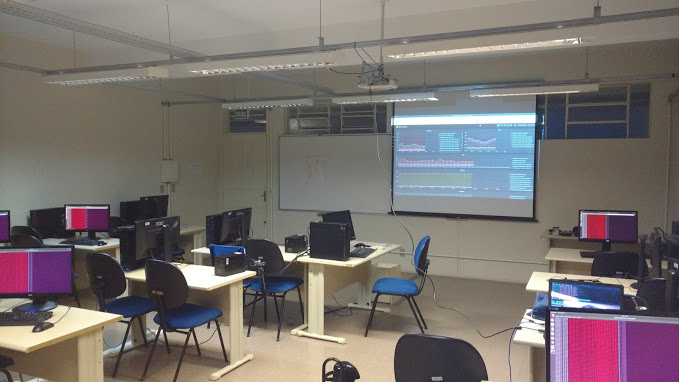
\includegraphics[width=0.8\textwidth]{figuras/network/lab.jpg}
  \centering

  Fonte: O próprio autor.
\end{figure}

As unidades computacionais visíveis na Figura~\ref{fig:laboratorio} são compostas por:

\begin{itemize}
  \item \ac{cpu}: 8 Núcleos
  \item Memória: 16 GB
  \item Disco: 1TB
\end{itemize}

Para cada teste, todos os clientes são encerrados, colocando o parâmetro de escalabilidade para zero.
%
O crescimento das conexões é dada de forma automatizada por um script ruby, onde ele entra em um laço de repetição na qual irá incrementar em 1 a escala dos contêineres de teste até que cheguem em 100.

O distribuidor de carga utilizado para a operação de escalabilidade é o Round Robin, a qual incrementará um contêinerer do cliente para cada máquina até que todas as máquinas tenham o mesmo número de cliente.
%
Caso a execução do contêinerer termine com um status diferente de 1, ele é realocado novamente para a mesma máquina, porém esta situação não ocorreu durante os testes.

\subsection{Ambiente de Metricas}
\label{sec:ambiente_met}

O ambiente de métricas foi implantado na nuvem computacional, junto ao banco de dados e as arquiteturas de microsserviços, a fim de garantir um tempo de resposta menor, diminuindo o impácto de existir uma coleta das informações na arquitetura.
%
Os recursos computacionais alocados para este serviço foram:

\begin{itemize}
  \item \ac{cpu}: 4 Núcleos
  \item Memória: 8 GB
  \item Disco: 40GB
\end{itemize}

A arquitetura foi implantada sobre estes recursos utilizando a tecnologia Docker. Em especial, este ambiente era responsável por conter o banco de dados de métricas, serviços de monitoramento de erros e monitoramento de consumo de recursos.
%
Também foi implantado o monitoramento de conexões simultâneas, distância média, mínima e máxima dos jogadores conforme a sua região, a fim de monitorar se o teste estava executando como descrito no planejamento, visível na Figura~\ref{fig:lab_monitor}

\begin{figure}[htb!]
  \caption{Monitoramento de conexões simultâneas.}
  \label{fig:lab_monitor}
  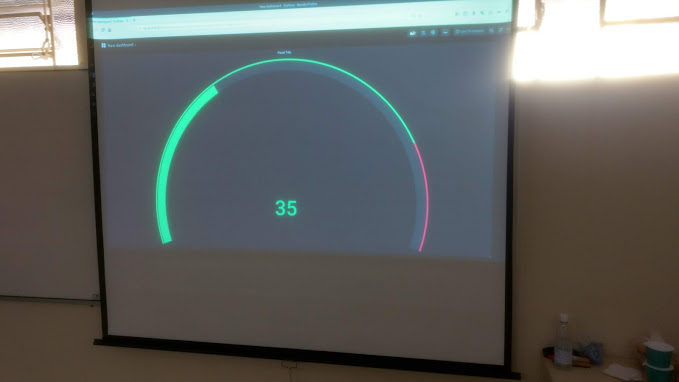
\includegraphics[width=0.8\textwidth]{figuras/network/metrics.jpg}
  \centering

  Fonte: O próprio autor.
\end{figure}

Durante os testes, utilizando o sistema de monitoramento das arquiteturas (visível nas Figuras~\ref{fig:lab_monitor, fig:laboratorio}),nenhum erro foi obtido nos conjuntos de dados utilizados para as análises.

\subsection{Interconexão entre Nuvem e Laboratório}
\label{sec:nuvem_lab}

A interconexão entre o laboratório e a nuvem computacional é um ponto de critério para a execução dos testes, visto que dada a capacidade e eficiência do tráfego de dados entre as duas redes, pode-se existir um gargalo limitador para os testes.
%
Este ponto deverá ser analisado, validando a vasão máxima entre as arquiteturas de microsserviços e os clientes.
